% ------------------------------------------------------------------------------
% TYPO3 Version 10.0 - What's New (Serbian Version)
%
% @author	Michael Schams <schams.net>
% @license	Creative Commons BY-NC-SA 3.0
% @link		http://typo3.org/download/release-notes/whats-new/
% @language	Serbian
% ------------------------------------------------------------------------------

\section{Uvod}
\begin{frame}[fragile]
	\frametitle{Uvod}

	\begin{center}\huge{Uvod}\end{center}
	\begin{center}\huge{\color{typo3darkgrey}\textbf{Cinjenice}}\end{center}

\end{frame}

% ------------------------------------------------------------------------------
% TYPO3 Version 10.0 - The Facts

\begin{frame}[fragile]
	\frametitle{Uvod}
	\framesubtitle{TYPO3 Verzija 10.0 - Cinjenice}

	\begin{itemize}
		\item Datum objavljivanja: 23. Jul 2019.
		\item Tip objavljivanja: Brza objava (Sprint Release)
		\item Vreme razvoja: oko 6 meseci
	\end{itemize}

	\begin{figure}
		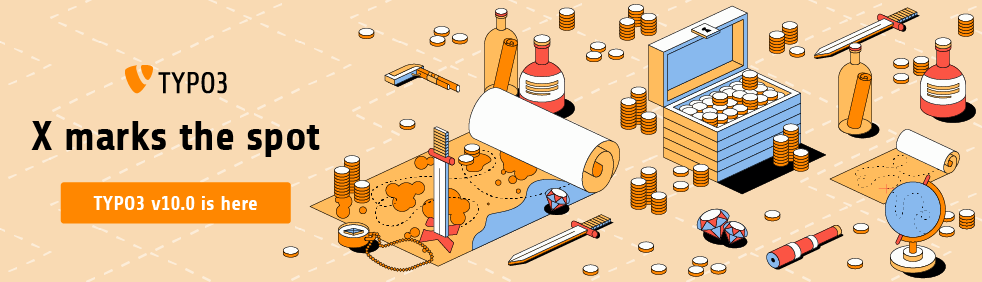
\includegraphics[width=0.95\linewidth]{Introduction/typo3-v10-0-banner.png}
	\end{figure}

\end{frame}

% ------------------------------------------------------------------------------
% TYPO3 Version 10.0 - Executive Summary

\begin{frame}[fragile]
	\frametitle{Uvod}
	\framesubtitle{Rezime}

	\small
		TYPO3 verzija 10.0 je prva brza objava na putu ka LTS-verziji
		(verzija sa dugorocnom podrškom) u 2020.

		\vspace{0.2cm}

		S obzirom da je fokus verzije 10.0 na precišcavanju koda, ne treba da zacudi
		veliki broj korenitih promena (breaking changes).

		\vspace{0.2cm}

		Ovakav pristup omogucava da se dodaju nove biblioteke koda, moderni koncepti
		i aktuelni API-ji u ranoj fazi razvoja da bi se omogucilo da TYPO3 ostane jedan
		od najboljih sistema za upravljanje sadržajem na tržištu.
		\vspace{0.2cm}

		Veliki broj uzbudljivih
		\href{https://typo3.org/community/teams/typo3-development/initiatives/}{inicijativa}
		je sastavljen da omoguci dugorocna unapredjenja u okviru TYPO3 sistema za upravljanje sadržajem.
	\normalsize

\end{frame}

% ------------------------------------------------------------------------------
% System Requirements

\begin{frame}[fragile]
	\frametitle{Uvod}
	\framesubtitle{Sistemski zahtevi}

	\begin{itemize}
		\item PHP verzija 7.2 ili 7.3
		\item PHP podešavanja:

			\begin{itemize}
				\item \texttt{memory\_limit} >= 256M
				\item \texttt{max\_execution\_time} >= 240s
				\item \texttt{max\_input\_vars} >= 1500
				\item opcija \texttt{-}\texttt{-disable-ipv6} \underline{ne sme} se koristit
			\end{itemize}

		\item Vecina DB servera koji rade sa \textbf{Doctrine DBAL} rade takodje i sa TYPO3.
			Testirani DB serveri su:
	\end{itemize}

	\begin{figure}
		
\includegraphics[width=0.80\linewidth]{Introduction/logo-databases.png}
	\end{figure}

\end{frame}

% ------------------------------------------------------------------------------
% Development, Release and Maintenance Timeline

\begin{frame}[fragile]
	\frametitle{Uvod}
	\framesubtitle{Razvoj, objavljivanje i vreme održavanja}

	\textbf{TYPO3 v10}

	\begin{figure}
		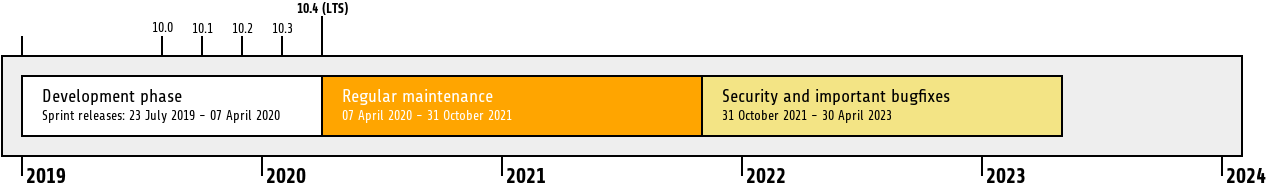
\includegraphics[width=1\linewidth]{Introduction/typo3-v10-lifecycle.png}
	\end{figure}

	\textbf{Produženo vreme podrške}\newline
	\smaller
		\href{https://typo3.com}{TYPO3 GmbH} nudi dodatne opcije za podršku za
		TYPO3 v10 LTS cak i posle 30. Aprila 2023. za dodatne dve godine.
	\normalsize

\end{frame}

% ------------------------------------------------------------------------------
% TYPO3 v10 Roadmap

\begin{frame}[fragile]
	\frametitle{Uvod}
	\framesubtitle{TYPO3 v10 plan}

	Predvidjeni datumi objavljivanja i njihov osnovni fokus:

	\begin{itemize}

		\item
			\begingroup
				\color{typo3orange}
				v10.0 \tabto{1.1cm}23/Jul/2019\tabto{3.4cm}Otvaranje puta za uzbudljive nove koncepte i API-je
			\endgroup
		\item v10.1 \tabto{1.1cm}01/Okt/2019\tabto{3.4cm}Unapredjenje routing-a i upravljanje sajtom v2
		\item v10.2 \tabto{1.1cm}03/Dec/2019\tabto{3.4cm}Fluid/Rendering Engine unapredjenja
		\item v10.3 \tabto{1.1cm}04/Feb/2020\tabto{3.4cm}Zamrzavanje funkcionalnosti
		\item v10.4 \tabto{1.1cm}07/Apr/2020\tabto{3.4cm}LTS objava (objava sa dugorocnom podrškom)

	\end{itemize}

	\smaller
		\url{https://typo3.org/article/typo3-v10-roadmap/}\newline
		\url{https://typo3.org/article/typo3-v10-safe-and-sound/}
	\normalsize

\end{frame}

% ------------------------------------------------------------------------------
% Installation

\begin{frame}[fragile]
	\frametitle{Uvod}
	\framesubtitle{Instalacija}

	\begin{itemize}
		\item Zvanicna \textit{klasicna} procedura za instalaciju na Linux/Mac OS X\newline
			(DocumentRoot na primer \texttt{/var/www/site/htdocs}):
		\begin{lstlisting}
$ cd /var/www/site
$ wget --content-disposition get.typo3.org/10.0
$ tar xzf typo3_src-10.0.0.tar.gz
$ cd htdocs
$ ln -s ../typo3_src-10.0.0 typo3_src
$ ln -s typo3_src/index.php
$ ln -s typo3_src/typo3
$ touch FIRST_INSTALL
		\end{lstlisting}

		\item Simbolicki linkovi (Symbolic links) na Microsoft Windows:

			\begin{itemize}
				\item Koristiti \texttt{junction} za Windows XP/2000
				\item Koristiti \texttt{mklink} za Windows Vista, Windows 7 i novije
			\end{itemize}

	\end{itemize}
\end{frame}

% ------------------------------------------------------------------------------
% Installation using composer

\begin{frame}[fragile]
	\frametitle{Instalacija i ažuriranje}
	\framesubtitle{Instalacija korišcenjem \texttt{composer-a}}

	\begin{itemize}
		\item Instalacija korišcenjem \textit{composer-a} na Linux/Mac OS X i Windows 10:

			\begin{lstlisting}
$ cd /var/www/site/
$ composer create-project typo3/cms-base-distribution typo3v10 ^10
			\end{lstlisting}

		\item Alternativno, napravite Vaš \texttt{composer.json} fajl i pokrenite:

			\begin{lstlisting}
$ composer install
			\end{lstlisting}

			Više detalja i primer \texttt{composer.json} fajla možete skinuti sa:\newline
			\smaller
				\href{https://composer.typo3.org}{https://composer.typo3.org}
			\normalsize

	\end{itemize}
\end{frame}

% ------------------------------------------------------------------------------
